To calculate the effect of magnetic permeability on magnetic materials, this paper uses the magnetic charge model \cite{Furlani2001}, where fictitious magnetic charges exist on the surface of and inside magnetic bodies. An example of this is depicted in Figure \ref{fig:p4singleMagnetPicture}, where an idealised permanent magnet with unity relative permeability \(\mu_r = 1\) and a non-ideal permanent magnet with \(\mu_r = 3\) have been drawn, with positive charges shown in red and negative charges in blue. Both magnets have identical remanence magnetisations, but the non-ideal magnet has a demagnetising effect on itself due to a relatively large value of permeability, resulting in weaker surface charges and some charges migrating from the north and south poles to the sides of the magnet. For non-unity relative permeability, the distributions of magnetic charge on the magnet surfaces is unknown and must be solved based on their interaction with each other and any applied magnetic field. This section outlines an approach to calculating these charge densities which uses a one-step matrix inversion rather than the iterative approach commonly seen in literature.
\begin{figure}
    \centering
    \begin{subfigure}{0.7\textwidth}
        \centering
        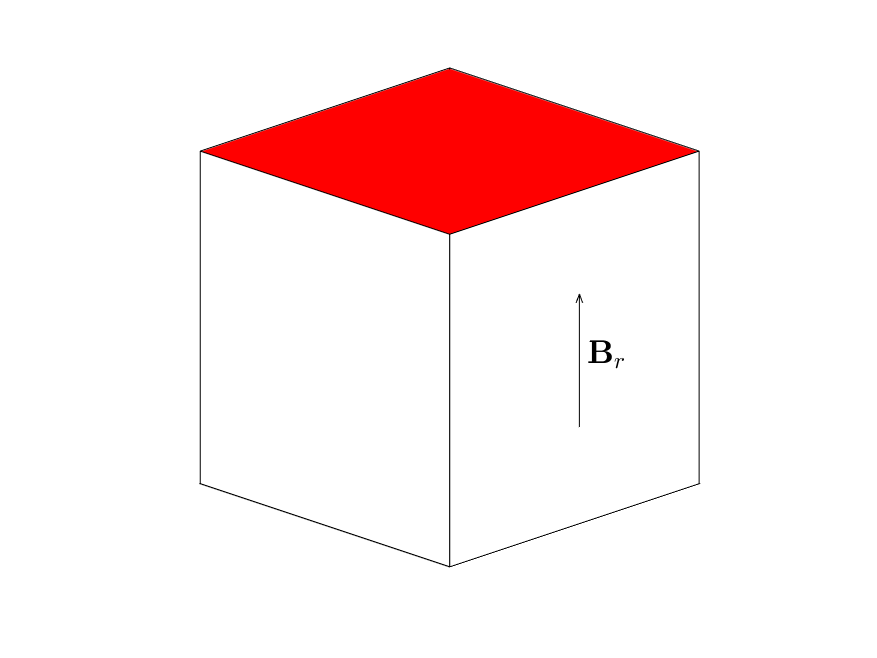
\includegraphics[width=\linewidth]{p4/p4FIG1a}
        \caption{}\label{fig:p4singleMagnetIdealised}
    \end{subfigure}
    \begin{subfigure}{0.7\textwidth}
        \centering
        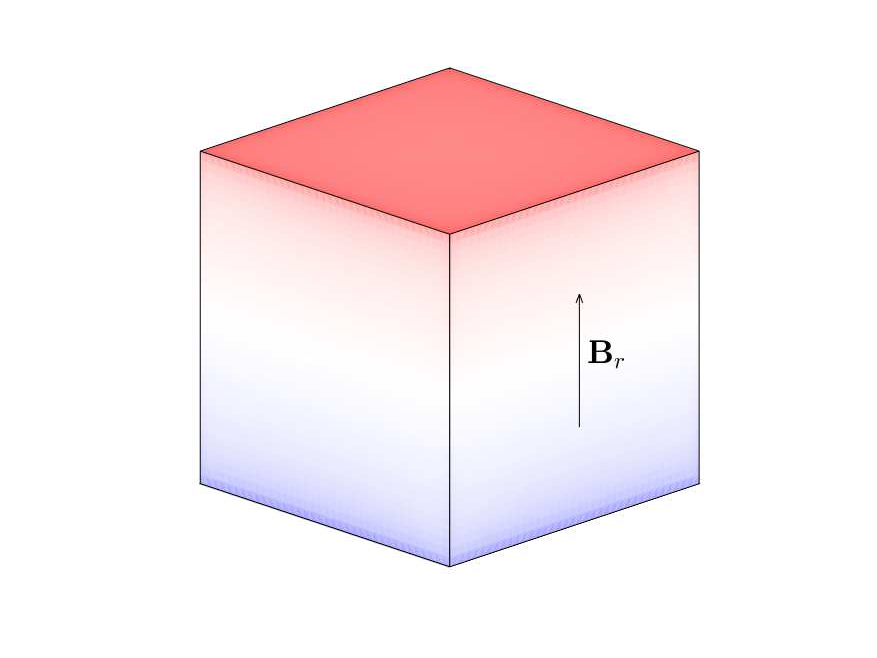
\includegraphics[width=\linewidth]{p4/p4FIG1b}
        \caption{}\label{fig:p4singleMagnetNonideal}
    \end{subfigure}
    \caption{A cube magnet with an ideal relative permeability \(\mu_r = 1\) (a) and a non-ideal relative permeability \(\mu_r = 3\) (b). The remanence magnetisation of both magnets is equal in strength and in the vertical direction, with the associated surface charges shown in red (positive charge) and blue (negative charge). The surface charges on the idealised magnet (\(\mu_r = 1\)) remain on the poles, whereas the charges on the non-ideal magnet (\(\mu_r = 3\)) migrate from the poles and become weaker due to the self-demagnetising effect of relatively large permeability.}
    \label{fig:p4singleMagnetPicture}
\end{figure}
%
\subsection{Induced magnetisation and surface charge density}
At any point in space, magnetic materials satisfy the constitutive relationship
\begin{equation}\label{eqn:p4constitutiveRelation}
    \mathbf{B} = \mu_0 \left( \mathbf{H} + \mathbf{M} \right)
\end{equation}
and Gauss' law for magnetism
\begin{equation}\label{eqn:p4gaussLawForMagnetism}
    \oiint_S \mathbf{B} \cdot d\mathbf{s}' \text{,}
\end{equation}
where \(\mathbf{B}\) is the magnetic flux density, \(\mu_0\) is the permeability of free space, \(\mathbf{H}\) is the magnetic field intensity, \(\mathbf{M}\) is the magnetisation of the material, and \(S\) is any closed surface in space. In addition, if the material is linear with a constant permeability \(\mu\), the flux density follows
\begin{equation}\label{eqn:p4linearMaterial}
    \mathbf{B} = \mu \mathbf{H} + \mathbf{B}_r \text{,}
\end{equation}
where \(\mathbf{B}_r\) is the remanence magnetisation of the material.

Combining Equations (\ref{eqn:p4constitutiveRelation}) and (\ref{eqn:p4linearMaterial}) leads to the equivalent magnetisation
\begin{equation}\label{eqn:p4equivalentMagnetisation}
    \mathbf{M} = \frac{1}{\mu} \mathbf{B}_r + \frac{\mu_r - 1}{\mu} \mathbf{B} \text{,}
\end{equation}
where \(\mu_r = \mu / \mu_0\) is the relative permeability of the material (with magnetic susceptibility \(\chi = \mu_r - 1\)). Thus, if the magnetic flux density is calculated and the remanence magnetisation known, the equivalent magnetisation can be calculated.

To solve Equation (\ref{eqn:p4equivalentMagnetisation}), an expression for the magnetic flux density \(\mathbf{B}\) must be found. Here, the magnetic charge model is used due to its accuracy and simplicity, but a number of other methods may be used. The magnetic flux density produced by a volume \(V\) bounded by a surface \(S\) at a location \(\mathbf{x}\) is presented by \textcite{Furlani2001} (pp. 132),
\begin{align}\label{eqn:p4chargeModel}
    \mathbf{B}\left( \mathbf{x} \right) = \frac{\mu_0}{4\pi} & \left( \oiint_{S} \left( \mathbf{M} \cdot \hat{\mathbf{n}} \right) \frac{\mathbf{x} - \mathbf{x}'}{\left| \mathbf{x} - \mathbf{x}' \right|^3} \ ds' - \iiint_{V} \left( \nabla \cdot \mathbf{M} \right) \frac{\mathbf{x} - \mathbf{x}'}{\left| \mathbf{x} - \mathbf{x}' \right|^3} \ dv' \right) \text{,}
\end{align}
where \(\mathbf{M}\) is the magnetisation of the volume, \(\hat{\mathbf{n}}\) is the outward-facing unit normal vector of the surface \(S\), and \(\mathbf{x}'\) is a point on \(S\) or in \(V\).

If each volume \(V\) is assumed to have constant uniform remanence magnetisation and constant permeability, \(\nabla \cdot \mathbf{M} = 0\) (Appendix \ref{sec:p4noVolumeCharge}) and the volume integral in Equation (\ref{eqn:p4chargeModel}) disappears, leaving the simplified charge model
\begin{align}\label{eqn:p4simplifiedChargeModel}
    \mathbf{B}\left( \mathbf{x} \right) = \frac{\mu_0}{4\pi} \oiint_{S} \sigma \left( \mathbf{x}' \right) \frac{\mathbf{x} - \mathbf{x}'}{\left| \mathbf{x} - \mathbf{x}' \right|^3} \ ds' \text{,}
\end{align}
where \(\sigma = \mathbf{M} \cdot \hat{\mathbf{n}}\) is the magnetic surface charge density.

Combining Equations (\ref{eqn:p4equivalentMagnetisation}) and (\ref{eqn:p4simplifiedChargeModel}) gives the equivalent magnetisation
\begin{equation}\label{eqn:p4badMagnetisationEquation}
    \mathbf{M} = \frac{1}{\mu} \mathbf{B}_r + \frac{\mu_r - 1}{\mu} \frac{\mu_0}{4\pi} \oiint_{S} \sigma \left( \mathbf{x}' \right) \frac{\mathbf{x} - \mathbf{x}'}{\left| \mathbf{x} - \mathbf{x}' \right|^3} \ ds' \text{.}
\end{equation}
To more easily analyse the system, a scalar equation may be employed using the scalar surface charge density rather than the magnetisation vector field. The equivalent surface charge density \(\sigma \left( \mathbf{x} \right)\) can be found by calculating the dot product of Equation (\ref{eqn:p4badMagnetisationEquation}) and the outward-facing unit normal vector \(\hat{\mathbf{n}}\),
\begin{align}\label{eqn:p4analyticSigma}
    \sigma \left( \mathbf{x} \right) = \frac{1}{\mu_r} \sigma_r + \frac{\mu_r - 1}{\mu} \frac{\mu_0}{4\pi} \oiint_{S} \sigma \left( \mathbf{x}' \right) \frac{\mathbf{x} - \mathbf{x}'}{\left| \mathbf{x} - \mathbf{x}' \right|^3} \ ds' \cdot \hat{\mathbf{n}} \text{,}
\end{align}
where \(\sigma_r = \mathbf{B}_r/\mu_0 \cdot \hat{\mathbf{n}}\) is defined as the remanence surface charge density.

Solving \(\sigma\) using Equation (\ref{eqn:p4analyticSigma}) is difficult, because \(\sigma\) is present both inside and outside of the integral. This problem suggests an iterative approach to solving \(\sigma\), such as in \cite{Casteren2014}. However, this issue can be avoided by applying a surface mesh to \(S\), as is shown in the following sections.

\subsection{Surface mesh}
By applying a surface mesh with \(N\) elements to \(S\), each surface element can be considered separately with its own surface charge density. When applied to a surface \(S\), Equation (\ref{eqn:p4gaussLawForMagnetism}) implies that (Appendix \ref{sec:p4integralSigma})
\begin{equation}
    \oiint_S \sigma \left(\mathbf{x}\right) ds = 0 \text{.}
\end{equation}
After meshing the surface and assuming that \(\sigma_i\) is constant across each surface, we obtain
\begin{equation}\label{eqn:p4sumOfSigmaEquation}
    \sigma_1 a_1 + \sigma_2 a_2 + \dots + \sigma_N a_N = 0 \text{,}
\end{equation}
where \(a_i\) is the area of the \(i\)th surface element. If Equation (\ref{eqn:p4sumOfSigmaEquation}) is false, the net magnetic charge of the system is non-zero, leading to inconsistency with Gauss' law. Thus, Equation (\ref{eqn:p4sumOfSigmaEquation}) will form a constraint on the solution of the magnetic system.

In addition, applying Equation (\ref{eqn:p4analyticSigma}) to the element \(i\) results in the definition of the surface charge density of each element \(\sigma_i\) as
\begin{align}
    \sigma_i \left( \mathbf{x}_i \right) &= \frac{1}{\mu_r} \sigma_{ir}\ + \frac{\mu_r - 1}{\mu} \sum_j \frac{\mu_0}{4\pi} \iint_{S_j} \sigma_j \left( \mathbf{x}_j' \right) \frac{\mathbf{x}_i - \mathbf{x}_j'}{\left| \mathbf{x}_i - \mathbf{x}_j' \right|^3} \ ds_j' \cdot \hat{\mathbf{n}}_i \text{,}
\end{align}
where \(\sigma_{ir}\) is the remanence surface charge density of element \(i\), \(\mathbf{x}_i\) is a point on element \(i\), and \(S_j\) is the surface of element \(j\).

If the surface mesh is chosen such that the surface charge density is approximately constant over each element, then \(\sigma_j \left( \mathbf{x}_j \right) \approx \sigma_j\), which can then be moved outside the integral,
\begin{align}\label{eqn:p4analyticSigmaDiscretised}
    \sigma_i \approx & \frac{1}{\mu_r} \sigma_{ir} + \frac{\mu_r - 1}{\mu} \sum_j \frac{\mu_0}{4\pi} \sigma_j \iint_{S_j} \frac{\mathbf{x}_i - \mathbf{x}_j'}{\left| \mathbf{x}_i - \mathbf{x}_j' \right|^3} \ ds_j' \cdot \hat{\mathbf{n}}_i \ \text{.}
\end{align}
The accuracy of each \(\sigma_i\) calculation increases as the mesh density increases. In addition, if a triangular surface mesh is used, any polyhedral geometry can be analysed this way, and curved surfaces may be approximated by a polyhedral surface with a large number of elements. This allows an accurate analysis of any magnetic geometry.

To simplify Equation (\ref{eqn:p4analyticSigmaDiscretised}), \(\hat{B}_{ij}\) is defined as
\begin{equation}\label{eqn:p4Bij}
    \hat{B}_{ij} = \frac{\mu_0}{4\pi} \iint_{S_j} \frac{\mathbf{x}_i - \mathbf{x}_j'}{\left| \mathbf{x}_i - \mathbf{x}_j' \right|^3} \ ds_j' \cdot \hat{\mathbf{n}}_i \text{,}
\end{equation}
which is equal to the normal magnetic flux density produced by element \(j\) at the centre of element \(i\) due to a unit surface charge density. The integral has been solved for triangular and trapezial elements by the current authors in a previous publication \cite{OConnell2020a}, and can be dot multiplied with the outward-facing normal vector to give \(\hat{B}_{ij}\). Note that to most efficiently calculate the force and torque in Section \ref{sec:p4forceAndTorque}, it is best to calculate the integral and store the result in \(\hat{B}_{xij}\), \(\hat{B}_{yij}\), and \(\hat{B}_{zij}\), before calculating the dot product. Substituting Equation (\ref{eqn:p4Bij}) into Equation (\ref{eqn:p4analyticSigmaDiscretised}) leads to 
\begin{equation}\label{eqn:p4sigmaApprox}
    \sigma_i \approx \frac{1}{\mu_r} \sigma_{ir} + \frac{\mu_r - 1}{\mu} \sum_j \hat{B}_{ij} \sigma_j \text{.}
\end{equation}

Equations (\ref{eqn:p4sumOfSigmaEquation}) and (\ref{eqn:p4sigmaApprox}) can be used to construct a matrix form of the problem, allowing the solution of all surface charge densities simultaneously. 

\subsection{Matrix equations}
It can be seen that Equations (\ref{eqn:p4sumOfSigmaEquation}) and (\ref{eqn:p4sigmaApprox}) represent a set of linear equations. Thus, we can write these equations as a set of matrix equations to manipulate and solve more easily. To do this, a vector of surface charge densities with length \(N\) is defined by
\begin{equation}
    \bm{\sigma} = \begin{bmatrix} \sigma_1 \\ \sigma_2 \\ \vdots \\ \sigma_N \end{bmatrix}
\end{equation}
with a similar vector of element surface areas given by
\begin{equation}
    \mathbf{a} = \begin{bmatrix} a_1 & a_2 & \dots & a_N \end{bmatrix} \text{,}
\end{equation}
Equation (\ref{eqn:p4sumOfSigmaEquation}) simplifies to
\begin{equation}\label{eqn:p4gaussLawMatrixEquation}
    \mathbf{a} \bm{\sigma} = 0 \text{.}
\end{equation}

To reduce Equation (\ref{eqn:p4sigmaApprox}) to a matrix equation, a matrix \(\hat{B}\) is defined by
\begin{equation}
    \hat{B} = \begin{bmatrix} \hat{B}_{11} & \hat{B}_{12} & \dots & \hat{B}_{1N} \\
    \hat{B}_{21} & \hat{B}_{22} & \dots & \hat{B}_{2N} \\
    \vdots & \vdots & \ddots & \vdots \\
    \hat{B}_{N1} & \hat{B}_{N2} & \dots & \hat{B}_{NN} \end{bmatrix} \nonumber \text{,}
\end{equation}
along with the remanence surface charge density vector,
\begin{equation}
    \bm{\sigma}_0 = \begin{bmatrix} \sigma_{1r} \\ \sigma_{2r} \\ \vdots \\ \sigma_{Nr} \end{bmatrix} \text{.}
\end{equation}
Thus, equation (\ref{eqn:p4sigmaApprox}) becomes the matrix equation
\begin{equation}\label{eqn:p4preIterativeEquation}
    \bm{\sigma} \approx K \bm{\sigma}_0 + J \hat{B} \bm{\sigma} \text{,}
\end{equation}
where
\begin{equation}
    K = \frac{1}{\mu_r}
\end{equation}
and
\begin{equation}
    J = \frac{\mu_r - 1}{\mu} \text{.}
\end{equation}
Assuming the matrix
\begin{equation}\label{eqn:p4CEquation}
    C = I - J \hat{B}
\end{equation}
is invertible (Appendix \ref{sec:p4invertibleMatrix}), where \(I\) is the \(\left(N\times N\right)\) identity matrix, Equation (\ref{eqn:p4preIterativeEquation}) can be rearranged to solve for all surface charge densities,
\begin{equation}\label{eqn:p4sigma}
    \bm{\sigma} \approx C ^{-1} K \bm{\sigma}_0 \text{.}
\end{equation}

Here, we have obtained an \(\left(N \times N\right)\) approximate matrix equation for the \(N\) surface charge densities in Equation (\ref{eqn:p4sigma}), with the constraint in Equation (\ref{eqn:p4gaussLawMatrixEquation}). This suggests using the method of constrained least squares, where
\begin{equation}
    \left| C\bm{\sigma} - K \bm{\sigma}_0 \right|^2
\end{equation}
is minimised, subject to the constraint \(\mathbf{a}\bm{\sigma} = 0\). This is done using the \( \left( N+1 \right) \times \left( N+1 \right)\) matrix equation
\begin{equation}
    \begin{bmatrix} 2C^\mathsf{T}C & \mathbf{a}^\mathsf{T} \\ \mathbf{a} & 0 \end{bmatrix} \begin{bmatrix} \bm{\sigma} \\ z \end{bmatrix} = \begin{bmatrix} 2C^\mathsf{T} K \bm{\sigma}_0 \\ 0 \end{bmatrix} \text{.}
\end{equation}
Thus, an accurate approximation for the surface charge densities which satisfy Gauss' Law for Magnetism is given by the first \(N\) elements of the solution to
\begin{equation}\label{eqn:p4singleMagnetSolution}
     \begin{bmatrix} \bm{\sigma} \\ z \end{bmatrix} = \begin{bmatrix} 2C^\mathsf{T}C & \mathbf{a}^\mathsf{T} \\ \mathbf{a} & 0 \end{bmatrix}^{-1} \begin{bmatrix} 2C^\mathsf{T} K \bm{\sigma}_0 \\ 0 \end{bmatrix} \text{.}
\end{equation}

While it is possible to simply solve Equation (\ref{eqn:p4sigma}) for the surface charge densities without the inclusion of Gauss' law, doing so often leads to a non-zero net surface charge density for the system. This is inconsistent with Gauss' law, and often leads to unbalanced forces and torques, violating Newton's third law. Since the inclusion of Gauss' law adds insignificant computation effort, it is beneficial to solve the constrained least squares problem given in Equation (\ref{eqn:p4singleMagnetSolution}) to ensure consistency with Maxwell's equations and improve accuracy of the final calculations.

\subsection{Multi-magnet systems}
In the previous sections, it is assumed that although the surface charge density \(\sigma_i\) of every element can vary, each element shares the same permeability \(\mu\). However, many magnetic systems consist of multiple magnetic objects, each with differing permeabilities. In this case, a small extension can be made to Equation (\ref{eqn:p4singleMagnetSolution}), allowing the calculation of the surface charge densities of magnetic objects with differing permeabilities. If \(J\) and \(K\) are redefined as the diagonal matrices
\begin{equation}\label{eqn:p4JEquation}
	J = \begin{bmatrix} \frac{\mu_{r1} - 1}{\mu_1} & 0 & \cdots & 0 \\
	0 & \frac{\mu_{r2} - 1}{\mu_2} & \cdots & 0 \\
	\vdots & \vdots & \ddots & \vdots \\
	0 & 0 & \cdots & \frac{\mu_{rN} - 1}{\mu_N} \end{bmatrix}
\end{equation}
and
\begin{equation}\label{eqn:p4KEquation}
	K = \begin{bmatrix} \frac{1}{\mu_{r1}} & 0 & \cdots & 0 \\
	0 & \frac{1}{\mu_{r2}} & \cdots & 0 \\
	\vdots & \vdots & \ddots & \vdots \\
	0 & 0 & \cdots & \frac{1}{\mu_{rN}} \end{bmatrix} \text{,}
\end{equation}
where \(\mu_n\) and \(\mu_{rn}\) are the permeability and relative permeability of element \(n\) respectively, the matrix \(C\) may be recalculated.

Once \(C\) is recalculated, Equation (\ref{eqn:p4singleMagnetSolution}) may be solved, but we can impose further constraints to yield a more accurate solution. Rather than applying Gauss' Law for Magnetism to the entire system, it can be applied to each magnet individually, giving one constraint per magnet. Given a system with \(M\) magnets, the area vector \(_m\mathbf{a}\) may be defined as
\begin{equation}
    _m\mathbf{a} = \begin{bmatrix} _ma_1 & _ma_2 & \dots \end{bmatrix} \text{,}
\end{equation}
where \(_ma_1\) is the area of the first element of magnet \(m\), \(_ma_2\) is the area of the second element of magnet \(m\), and so on. These area vectors may be formed into an \(M \times N\) block diagonal matrix \(A\), given by
\begin{equation}\label{eqn:p4AEquation}
    A = \begin{bmatrix} _m\mathbf{a} & \bm{0} & \bm{0} & \dots & \bm{0} \\
    \bm{0} & _2\mathbf{a} & \bm{0} & \dots & \bm{0} \\
    \bm{0} & \bm{0} & _3\mathbf{a} & \dots & \bm{0} \\
    \vdots & \vdots & \vdots & \ddots & \vdots \\
    \bm{0} & \bm{0} & \bm{0} & \dots & _M\mathbf{a} \end{bmatrix} \text{,}
\end{equation}
where each \(\bm{0}\) is a zero-values row vector. Applying Gauss' Law for Magnetism to each magnet in the system gives the new constraint
\begin{equation}
    A\bm{\sigma} = \bm{0} \text{.}
\end{equation}
This may be incorporated into the constrained least squares system, giving the solution to the \(\left(M+N\right)\times\left(M+N\right)\) linear system
\begin{equation}\label{eqn:p4multiMagnetSolution}
    \begin{bmatrix} \bm{\sigma} \\ z \end{bmatrix} = \begin{bmatrix} C^\mathsf{T}C & A^\mathsf{T} \\ A & 0 \end{bmatrix}^{-1} \begin{bmatrix} C^\mathsf{T} K \bm{\sigma}_0 \\ 0 \end{bmatrix} \text{.}
\end{equation}

One considerable advantage of this methodology is that the surface charges of several magnetic bodies may be solved simultaneously. Here, there is no need to calculate the effect of magnet 2 on magnet 1, then magnet 3 on magnet 1, and so on. Rather, the information of all magnetic bodies is encapsulated in the constrained least squares system, and the surface charge densities of the entire system may be solved with a single matrix inversion.

\subsection{External fields}\label{sec:p4externalFields}
Thus far in the derivation, only the fields generated by the magnetic bodies themselves have been considered; fields generated by other sources such as an electromagnetic coil or the Earth have not been incorporated. However, the methodology can be adapted to include these effects. The normal component of the external field \(\mathbf{B}_\text{ext}\) may be calculated at the centre of element \(n\) by calculating the dot product of the field at that point and the outward-facing unit normal vector, and is denoted by \(B_{\text{norm},n}\). An \(\left(N\times 1\right)\) vector can be defined by concatenating these normal field components, giving the vector of normal external fields,
\begin{equation}
    \mathbf{B}_\text{ext,norm} = \begin{bmatrix} B_{\text{norm},1} \\ B_{\text{norm},2} \\ \vdots \\ B_{\text{norm},N} \end{bmatrix} \text{.}
\end{equation}
This can be incorporated into the constrained least squares, giving the solution
\begin{equation}\label{eqn:p4externalMultiMagnetSolution}
    \begin{bmatrix} \bm{\sigma} \\ z \end{bmatrix} = \begin{bmatrix} C^\mathsf{T}C & A^\mathsf{T} \\ A & 0 \end{bmatrix}^{-1} \begin{bmatrix} C^\mathsf{T} \left( K \bm{\sigma}_0 + J\mathbf{B}_\text{ext,norm} \right) \\ 0 \end{bmatrix} \text{,}
\end{equation}
with \(J\), \(K\), \(C\), and \(A\) being defined by Equations (\ref{eqn:p4JEquation}), (\ref{eqn:p4KEquation}), (\ref{eqn:p4CEquation}), and (\ref{eqn:p4AEquation}) respectively.

\subsection{Summary}
This section has outlined a methodology for calculating the surface charge densities of magnetic surface elements assuming each element has a constant permeability and constant uniform remanence magnetisation. A surface mesh is applied to each magnetic body in a system, and a large matrix \(\hat{B}\) is defined. The \(\left(i,j\right)\) entry of \(\hat{B}\) is given by the normal component of the magnetic flux density at the centre of element \(i\) due to element \(j\), assuming element \(j\) has unity charge density. In addition, a vector \(\bm{\sigma}_0\) is defined as the initial surface charge densities of each element, diagonal matrices \(J\) and \(K\) initialised containing permeability information, and a block diagonal matrix \(A\) defined containing the area of each element. Finally, the surface charges \(\bm{\sigma}\) are solved using Equation (\ref{eqn:p4externalMultiMagnetSolution}). These surface charges are used in the following sections to calculate magnetic fields (Section \ref{sec:p4magneticField}), as well as forces and torques (Section \ref{sec:p4forceAndTorque}).